\chapter{Methodology}
This chapter should discuss the details of your implementation for the assignment. 
Everything related to \emph{how} things were done should go here.
Remember to avoid going into too much details, summarize appropriately and try to use figures/charts.
Make sure you refer to the figures (such as Figure \ref{fig:universe}) and charts you add in the text.
Avoid putting lots of source code here -- small code snippets are fine if you want to discuss something specific.

\begin{figure}
\centering
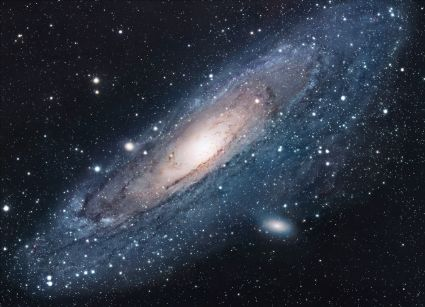
\includegraphics[scale=1.7]{images/universe.jpg}
\caption{A JPEG image of a galaxy. Use vector graphics instead if you can.}
\label{fig:universe}
\end{figure}

\section{Testing}
Add content in this section that describes how you tested and verified the correctness of your implementation, with respect to the requirements of the assignment.